\section*{\textbf{II. Experimental Design}}
\addcontentsline{toc}{section}{II.\hspace{0.15in} Experimental Design}

\hspace{0.15in}
The process of design for this experiment relies heavily on the use of a 15 milimeter right prism and our photonic crystal. The photonic crystal is composed of 3 bilayers of TiO2 and SiO2. The dielectric function of TiO2 is taken as $\epsilon_{TiO2} = 4.84 + 0.0007i$ and the dielectric function of SiO2 is taken as $\epsilon_{SiO2} = 2.1316 + 0.0001i$. 

\begin{wrapfigure}{R}{2in}
    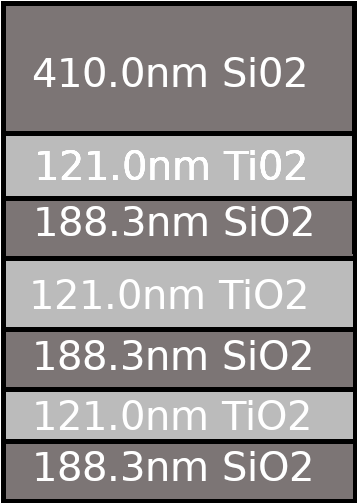
\includegraphics[width=2in]{multilayer.png}
    \caption{An illustration of the photonic crystal used in our sensor}
    \label{fig:multilayer}
\end{wrapfigure}

It should be noted that the imaginary parts of each dielectric function may not be accurate and have been included to introduce some form of loss that fits the results of prior experiments \cite{}. Figure 3 illustrates the structure of the multilayer.
The basic design of the sensor is split into three different parts: the primary stage, two beams, and the flowcell stage. The primary stage acts as the center about which the incident beam can be coupled to the prism and then reflected. One of the two beams holds our laser and a focusing lens while the other holds the CCD and captures the reflected beam. The flowcell stage is a modular piece that is attached to the primary stage with four bolts, the prism, multilayer, and flowcell chamber are all strapped together on this stage. The modular nature of this piece of the sensor is very valuable since many designs can be used to achieve the same goal and it only takes about an hour to print off each stage.\\
\vspace{0.1in}

% Picture of beams, central stage, and flowcell stage
\begin{figure}[h]
\end{figure}

To operate the sensor both beams need to be oriented at the \textit{coupling angle}. When the chamber is filled with water this angle is about $66^{\circ}$ from the surface of the prism. This is a rather extreme angle and so the parts that connect the beams to the rim of the primary stage are fashioned to allow the beams to pivot about their connection points. This allows the beams to be oriented at extreme angles with respect to the surface of the prism.